% Options for packages loaded elsewhere
\PassOptionsToPackage{unicode}{hyperref}
\PassOptionsToPackage{hyphens}{url}
\PassOptionsToPackage{dvipsnames,svgnames,x11names}{xcolor}
%
\documentclass[
  letterpaper,
  DIV=11,
  numbers=noendperiod]{scrartcl}

\usepackage{amsmath,amssymb}
\usepackage{iftex}
\ifPDFTeX
  \usepackage[T1]{fontenc}
  \usepackage[utf8]{inputenc}
  \usepackage{textcomp} % provide euro and other symbols
\else % if luatex or xetex
  \usepackage{unicode-math}
  \defaultfontfeatures{Scale=MatchLowercase}
  \defaultfontfeatures[\rmfamily]{Ligatures=TeX,Scale=1}
\fi
\usepackage{lmodern}
\ifPDFTeX\else  
    % xetex/luatex font selection
\fi
% Use upquote if available, for straight quotes in verbatim environments
\IfFileExists{upquote.sty}{\usepackage{upquote}}{}
\IfFileExists{microtype.sty}{% use microtype if available
  \usepackage[]{microtype}
  \UseMicrotypeSet[protrusion]{basicmath} % disable protrusion for tt fonts
}{}
\makeatletter
\@ifundefined{KOMAClassName}{% if non-KOMA class
  \IfFileExists{parskip.sty}{%
    \usepackage{parskip}
  }{% else
    \setlength{\parindent}{0pt}
    \setlength{\parskip}{6pt plus 2pt minus 1pt}}
}{% if KOMA class
  \KOMAoptions{parskip=half}}
\makeatother
\usepackage{xcolor}
\setlength{\emergencystretch}{3em} % prevent overfull lines
\setcounter{secnumdepth}{-\maxdimen} % remove section numbering
% Make \paragraph and \subparagraph free-standing
\makeatletter
\ifx\paragraph\undefined\else
  \let\oldparagraph\paragraph
  \renewcommand{\paragraph}{
    \@ifstar
      \xxxParagraphStar
      \xxxParagraphNoStar
  }
  \newcommand{\xxxParagraphStar}[1]{\oldparagraph*{#1}\mbox{}}
  \newcommand{\xxxParagraphNoStar}[1]{\oldparagraph{#1}\mbox{}}
\fi
\ifx\subparagraph\undefined\else
  \let\oldsubparagraph\subparagraph
  \renewcommand{\subparagraph}{
    \@ifstar
      \xxxSubParagraphStar
      \xxxSubParagraphNoStar
  }
  \newcommand{\xxxSubParagraphStar}[1]{\oldsubparagraph*{#1}\mbox{}}
  \newcommand{\xxxSubParagraphNoStar}[1]{\oldsubparagraph{#1}\mbox{}}
\fi
\makeatother


\providecommand{\tightlist}{%
  \setlength{\itemsep}{0pt}\setlength{\parskip}{0pt}}\usepackage{longtable,booktabs,array}
\usepackage{calc} % for calculating minipage widths
% Correct order of tables after \paragraph or \subparagraph
\usepackage{etoolbox}
\makeatletter
\patchcmd\longtable{\par}{\if@noskipsec\mbox{}\fi\par}{}{}
\makeatother
% Allow footnotes in longtable head/foot
\IfFileExists{footnotehyper.sty}{\usepackage{footnotehyper}}{\usepackage{footnote}}
\makesavenoteenv{longtable}
\usepackage{graphicx}
\makeatletter
\newsavebox\pandoc@box
\newcommand*\pandocbounded[1]{% scales image to fit in text height/width
  \sbox\pandoc@box{#1}%
  \Gscale@div\@tempa{\textheight}{\dimexpr\ht\pandoc@box+\dp\pandoc@box\relax}%
  \Gscale@div\@tempb{\linewidth}{\wd\pandoc@box}%
  \ifdim\@tempb\p@<\@tempa\p@\let\@tempa\@tempb\fi% select the smaller of both
  \ifdim\@tempa\p@<\p@\scalebox{\@tempa}{\usebox\pandoc@box}%
  \else\usebox{\pandoc@box}%
  \fi%
}
% Set default figure placement to htbp
\def\fps@figure{htbp}
\makeatother
% definitions for citeproc citations
\NewDocumentCommand\citeproctext{}{}
\NewDocumentCommand\citeproc{mm}{%
  \begingroup\def\citeproctext{#2}\cite{#1}\endgroup}
\makeatletter
 % allow citations to break across lines
 \let\@cite@ofmt\@firstofone
 % avoid brackets around text for \cite:
 \def\@biblabel#1{}
 \def\@cite#1#2{{#1\if@tempswa , #2\fi}}
\makeatother
\newlength{\cslhangindent}
\setlength{\cslhangindent}{1.5em}
\newlength{\csllabelwidth}
\setlength{\csllabelwidth}{3em}
\newenvironment{CSLReferences}[2] % #1 hanging-indent, #2 entry-spacing
 {\begin{list}{}{%
  \setlength{\itemindent}{0pt}
  \setlength{\leftmargin}{0pt}
  \setlength{\parsep}{0pt}
  % turn on hanging indent if param 1 is 1
  \ifodd #1
   \setlength{\leftmargin}{\cslhangindent}
   \setlength{\itemindent}{-1\cslhangindent}
  \fi
  % set entry spacing
  \setlength{\itemsep}{#2\baselineskip}}}
 {\end{list}}
\usepackage{calc}
\newcommand{\CSLBlock}[1]{\hfill\break\parbox[t]{\linewidth}{\strut\ignorespaces#1\strut}}
\newcommand{\CSLLeftMargin}[1]{\parbox[t]{\csllabelwidth}{\strut#1\strut}}
\newcommand{\CSLRightInline}[1]{\parbox[t]{\linewidth - \csllabelwidth}{\strut#1\strut}}
\newcommand{\CSLIndent}[1]{\hspace{\cslhangindent}#1}

\usepackage{booktabs}
\usepackage{longtable}
\usepackage{array}
\usepackage{multirow}
\usepackage{wrapfig}
\usepackage{float}
\usepackage{colortbl}
\usepackage{pdflscape}
\usepackage{tabu}
\usepackage{threeparttable}
\usepackage{threeparttablex}
\usepackage[normalem]{ulem}
\usepackage{makecell}
\usepackage{xcolor}
\usepackage{tabularray}
\usepackage[normalem]{ulem}
\usepackage{graphicx}
\UseTblrLibrary{booktabs}
\UseTblrLibrary{rotating}
\UseTblrLibrary{siunitx}
\NewTableCommand{\tinytableDefineColor}[3]{\definecolor{#1}{#2}{#3}}
\newcommand{\tinytableTabularrayUnderline}[1]{\underline{#1}}
\newcommand{\tinytableTabularrayStrikeout}[1]{\sout{#1}}
\KOMAoption{captions}{tableheading}
\makeatletter
\@ifpackageloaded{caption}{}{\usepackage{caption}}
\AtBeginDocument{%
\ifdefined\contentsname
  \renewcommand*\contentsname{Table of contents}
\else
  \newcommand\contentsname{Table of contents}
\fi
\ifdefined\listfigurename
  \renewcommand*\listfigurename{List of Figures}
\else
  \newcommand\listfigurename{List of Figures}
\fi
\ifdefined\listtablename
  \renewcommand*\listtablename{List of Tables}
\else
  \newcommand\listtablename{List of Tables}
\fi
\ifdefined\figurename
  \renewcommand*\figurename{Figure}
\else
  \newcommand\figurename{Figure}
\fi
\ifdefined\tablename
  \renewcommand*\tablename{Table}
\else
  \newcommand\tablename{Table}
\fi
}
\@ifpackageloaded{float}{}{\usepackage{float}}
\floatstyle{ruled}
\@ifundefined{c@chapter}{\newfloat{codelisting}{h}{lop}}{\newfloat{codelisting}{h}{lop}[chapter]}
\floatname{codelisting}{Listing}
\newcommand*\listoflistings{\listof{codelisting}{List of Listings}}
\makeatother
\makeatletter
\makeatother
\makeatletter
\@ifpackageloaded{caption}{}{\usepackage{caption}}
\@ifpackageloaded{subcaption}{}{\usepackage{subcaption}}
\makeatother

\usepackage{bookmark}

\IfFileExists{xurl.sty}{\usepackage{xurl}}{} % add URL line breaks if available
\urlstyle{same} % disable monospaced font for URLs
\hypersetup{
  pdftitle={Efekt rebalansiranja na Zagrebačkoj burzi},
  colorlinks=true,
  linkcolor={blue},
  filecolor={Maroon},
  citecolor={Blue},
  urlcolor={Blue},
  pdfcreator={LaTeX via pandoc}}


\title{Efekt rebalansiranja na Zagrebačkoj burzi}
\author{}
\date{}

\begin{document}
\maketitle


\section{Uvod}\label{uvod}

Domaći i inozemni investicijski investitori često održavaju fiksne
udjele dionica i obveznica u svom portfoliju. To se posebno odnosi na
mirovinske i državne fondove, koji ciljaju određenu strukturu portfolia,
poput poznatog 60 - 40 omjera (60 \% dionice, 40 \% obveznice). Ovi
fondovi često imaju i zakonska ograničenja ulaganja u pojedini tip
imovinske klase. Primjerice u RH postoji Pravilnik o dozvoljenim
ulaganjima i dodatnim ograničenjima ulaganja obveznog mirovinskog fonda,
koji utvrđuje maksimalno dopuštenja ulaganja u domaće i inozemne
dionice, obveznice, nekretnine i druge imovinske klase.

Ako tijekom određenog razdoblja jedna klasa imovine relativno raste u
odnosu na drugu klasu imovine, fondovi prodaju imovinsku klasu koja je
ostvarila bolje performanse i kupuju klasu imovine koja je ostvarila
lošije performanse. Cilj je dosegnuti unaprijed utvrđene pondere u
portfoliju. Fondovi dakle moraju kupovati gubitnike i prodavati
dobitnike, što može imati utjecaj na agregatna kretanja dioničkih i
obvezničkih tržišta. Rad upravo analizira mogući utjecaj rebalansiranja
mirovinskih, državnih i drugih fondova na agregatna kretanja dioničkog i
obvezničkog tržišta u RH. Pri tome je dinamika dioničkog tržišta
reprezentirana kretanjem dioničkog CROBEX indeksa, a kretanje
obvezničkog tržišta kretanje obvezničkog CROBIS indeksa.

Politika rebalansiranja investicijskih fondova, može se provoditi prema
dva pravila: kalendarsko pravilo i granično pravilo Doe (2025). Prema
graničnom pravilu, fondovi provode balansiranje kada udio određene
imovinske klase prijeđe određenu, unaprijed utvrđenu granicu. Dopušta se
fluktuacija unutar tih utvrđenih granica, ali ako pojedina klasa imovine
naraste značajno iznad određene granice, fond kupuje gubitnike i prodaje
dobitnike. Ideja je da se smanje transakcijski troškovi zbog (pre)čestog
trgovanja. Prema kalendarskom pravilu, fondovi provode rebalansiranje u
jednakim vremenskim intervalima. Najčešće je mjesečno rebalansiranje,
iako neki fondovi mogu koristiti kvartalno ili dnevno rebalansiranje. U
ovom radu se ispituje kalendarski efekt, odnosno utjecaj rebalansiranja
na kraju mjeseca na kretanje dioničkog i obvezničkog indeksa. Ako
postoji znatno rebalansiranje na kraju mjeseca, očekuje se rast prinosa
imovine s relativno slabijim performansama u prvom dijelu mjeseca i,
obrnuto, pad prinosa imovine koja je rasla u prvom dijelu mjeseca.
Razlog za mjesečno rebalansiranje može biti potreba za novčanim tokovima
na kraju mjeseca Etula et al. (2020). Da bi se utvrdilo točno vrijeme
rebalansiranja, nužno je raspolaganje dnevnim podacima o rebalansiranju
od investicijskih fondova. Takvi podaci nisu javno dostupni pa se
pretpostavlja mjesečno balansiranje koje je najčešći oblik
rebalansiranja.

Rebalansiranje može uzrokovati velike transakcije troškove za fondove.
Transakcijski troškovi obuhvaćaju brokerske provizije, \emph{bid-ask
spreadove} i tržišni utjecaj. Prečesto rebalansiranje stoga može imati
negativan utjecaj na profitabilnost investicijskih fondova. Postojanje
kalendarskog efekta može stoga upućivati na preveliki trošak
investiranja, te bi se moglo preporučiti promjena politike
rebalansiranja, ako je efekt ekonomski signifikantan. Efekt je važan i
za sofisticiranje i institucionalne investitore, koji mogu koristiti
informaciju o rebalansiranju za optimizaciju svojih investicijskih
strategija. Primjerice, ako netko želi kupiti dionice, bolje je da to
učini zadnji tjedan u mjesecu, ako je dionički indeks bio relativno
slabiji u prvom dijelu mjeseca.

Metodološki, utjecaj kalendarskog rebalansiranja analizira se s pomoću
tri pristupa. Prvo se provodi deskriptivna analiza kako bi se bi
utvrdile razlike u prosječnim prinosa CROBEX-a i CROBIS-a u posljednjih
5 trgovinskih dana uvjetovano na prinose u prvih 15 trgovinskih dana.
Potom se provodi regresijska analiza koja ispituje statistički odnos
između razlike prinosa CROBEX-a i CROBIS-a u prvih 15 trgovinskih dana i
posljednjih 5 trgovinskih dana. U trećem dijelu se provodi investicijski
pristup u kojem se utvrđuju ekonomski efekti rebalansiranja. Ispituje se
profitabilnost investicijske strategije koja kupuje podcijenjenu imovinu
5 trgovinskih dana prije kraja mjeseca. Kada je CROBEX relativno
podcijenjen u odnosu na dinamiku CROBIS-a, kupuje se CROBEX i obrnuto.

Rezultati pokazuju postojanje kalendarskog efekta. Regresija razlike
prinosa pokazuje negativan odnos, što potvrđuje efekt rebalansiranja.
Investicijska strategija koja kupuje podcijenjenu imovinu 5 dana prije
kraja mjeseca ostvaruje značajno bolje rezultate od strategije koja
uvijek drži CROBEX ili CROBIS zadnjih 5 dana u mjesecu ili tijekom
cijelog razdoblja. Sharpovi omjeri su duplo veći u odnosu na strategiju
kupi i drži CROBEX.

U analizi robusnosti testira se osjetljivost rezultata na 2 promjene u
analizi. Prvo, procjenjuje se efekt rebalansiranja na početku mjeseca
umjesto na kraju mjeseca. Izračunava prinos CROBEX-a i CROBIS-a u
posljednjih 15-ak trgovinskih dana u mjesecu, te se potom na početku
sljedećeg mjeseca kupuje imovina koja je ostvarila relativno manji
prinos. Potom se, slijedeći metodološki pristup osnovne analize, provodi
regresijska analiza i simulira investicijska strategija na povijesnim
podacima. Rezultati pokazuju da ovakva strategija ostvaruje znatno
lošije rezultate od bazične strategije koja kupuje relativno
podcijenjenu imovinu 5 dana prije kraja mjeseca. Regresijska analiza
pokazuje suprotan efekt u odnosu na bazičan model.

Drugi dio analize robusnosti analizira utjecaj pomaka u broju dana od
kraja mjeseca prema sredini mjeseca. Utvrđuje se utjecaj na rezultat s
obzirom na pomak varijable od 2 do 10 dana od kraja prema sredini
mjeseca. U ovom dijelu se provodi samo pristup investicijske strategije.
Analizira se razlika u Sharpovom omjeru i analiziranom prinosu
investicijske strategije u odnosu na bazičnu strategiju. Rezultati
pokazuju da se najbolji rezultati postižu kada se kupuje podcijenjena
imovina 5 dana prije kraja mjeseca. Sharpeov omjer se smanjuje kako se
broj dana smanjuje ili povećava, ali je konzistentno veći od Sharpeov
omjera CROBEX indeksa po principu kupi i drži.

Rezultati istraživanja mogu imati šire implikacije za razumijevanje
agregatnih tržišnih kretanja te pomoći investitorima u optimizaciji
svojih strategija ulaganja. Uz to, rad može poslužiti kao empirijska
osnova za donošenje regulatornih odluka i oblikovanje pravila
upravljanja portfeljima fondova u kontekstu hrvatskog financijskog
tržišta.

\section{Pregled literature}\label{pregled-literature}

Rad ima doprinos za dvije grupe istraživanja. Prvo je rastuća grupa
istraživanja koja se bavi utjecajem politika rebalansiranja
investicijskih fondova na tržišne nesavršenosti. Ovaj fenomen se počeo
snažnije proučavati posljednjih nekoliko godina Da et al. (2018) su
analizirali kako koordinirano trgovanje na temelju financijskih savjeta
može uzrokovati nestabilnost na tržištu. Studija analizira kako
preporuke tvrtke Felices y Forrados (FyF) o preusmjeravanju ulaganja
između dioničkih i obvezničkih fondova utječu na volatilnost tržišta i
alokaciju imovine mirovinskih fondova. Peng and Wang (2024) uvode
koncept faktorskog rebalansiranja, koji istražuje kako promjena
faktorske izloženosti utječe na rebalansiranje i povrate dionica.
Studija pokazuje da uzajamni fondovi imaju konstantnu potražnju za
faktorskom izloženošću (faktor veličine, vrijednosti, momentuma i
slično), te da promjene u faktorskoj izloženosti dovodi do pritisaka
prodaje određene dionice, kako bi se faktorska izloženost vratila u
ravnotežu. Parker, Schoar, and Sun (2022) analiziraju TDF fondove (eng.
Target Date Funds), koji automatski prilagođavaju alokaciju imovine na
temelju starosti investitora, postupno smanjujući izloženost dionicama u
korist obveznica kako se približava mirovina. Autori pokazuju kako
rebalansiranja TDF fondova djeluju kontrarijski, prodajući dionice nakon
razdoblja snažnih tržišnih performansi i kupnjom nakon pada tržišta,
djelujući suprotno dominantnim tržišnim trendovima. Politikom
rebalansiranja utječu i na dinamiku prostornih (eng. cross-section)
prinosa dionica. U Hrvatskoj je istraživan utjecaj vlasništva
institucionalnih investitora na uspješnost i financijsku poziciju
hrvatskih poduzeća Đunđek Kokotec, Orsag, and Klačmer Čalopa (2021).
Rezultati pokazuju statistički značajan utjecaj vlasništva
institucionalnih investitora na poslovnu uspješnost i financijsko
zdravlje poduzeća.

Druga grupa istraživanja se odnosi na radove koji su analizirali
pritiske cijena (eng. \emph{price pressure}). Rani doprinos dao je
Shleifer (1986), koji istražuje nagib krivulja potražnje za pojedinačnim
dionicama analizirajući cjenovne efekte prilikom uvrštavanja dionica u
dionički indeks. Sličnu analizu su proveli Harris and Gurel (1986) koji
su pokazali da cijene dionica rastu prilikom dodavanja i padaju prilikom
uklanjanja dionica iz indeksa, što podupire hipotezu o cjenovnim
pritiscima.

\section{Podaci i metode}\label{podaci-i-metode}

U rujnu 2024. godine imovina mirovinskih fondova u RH činila je 61 \%
ukupne vrijednosti imovine sektora financijskih usluga (Hrvatska
agencija za razvoj financijskih usluga (HANFA) (2025)). Po veličini
slijedi sektor osiguranja s 15 \%, dok investicijski fondovi i leasing
društva čine 11 \%. Postoji jasan trend rasta udjela mirovinskih
fondova. U 2017. godini udio imovine mirovinskih fondova je bio 52 \%.
Dakle u 7 godina udio imovine mirovinskih fondova je porastao za 9
postotnih poena. što potvrđuje značaj mirovinskih fondova u hrvatskom
financijskom sustavu.

\begin{figure}

\centering{

\pandocbounded{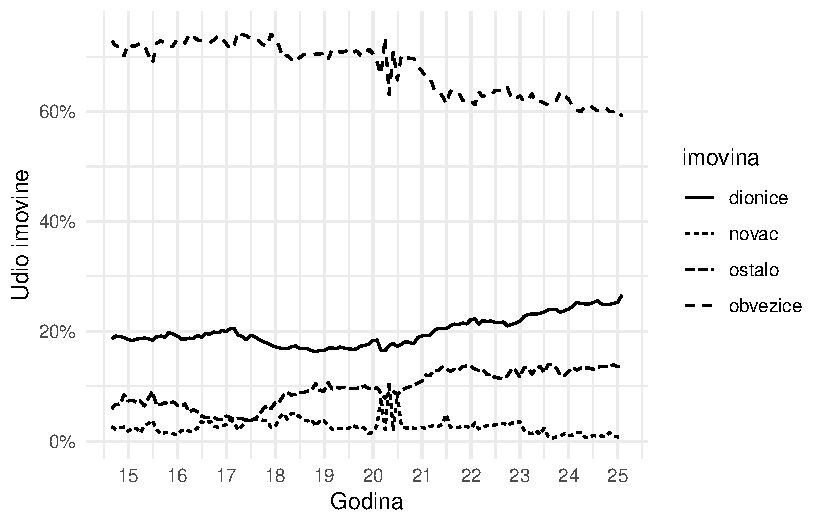
\includegraphics[keepaspectratio]{zse_eom_rebalansiranje_files/figure-pdf/fig-mf-1.pdf}}

}

\caption{\label{fig-mf}Struktura imovine mirovinskih fondova}

\end{figure}%

Zbog veličine i značaja mirovinskih fondova, važno je pratiti strukturu
njihove imovine. U tablici Figure~\ref{fig-mf} imovina mirovinskih
fondova podijeljena je u 4 kategorije: dionice, obveznice, novčana
sredstava i ostalo. Sumirane su stavke za sve oblike mirovinskih
fondova: obvezne mirovinske fondove te otvorene i zatvorene dobrovoljne
mirovinske fondove. U tablici se prikazuje udio svake imovinske klase u
ukupnoj imovini mirovinskih fondova. Od 2014. godine do 2021. godine
odnos dionica i obveznica je relativno stabilan. Mirovinski fondovi oko
20 \% imovine drže u dionicama i oko 70 \% imovine u obveznicama.
Tijekom 2021. godine omjeri su se promijenili. Udio obveznica je pao na
otprilike 50 \%. Treba napomenuti i da je 2024. stupio na snagu novi
zakon koji je smanjio zakonsko ograničenje ulaganja u državne obveznice
s 50 \% na 45\%.

Može se zaključiti da zakonska ograničenja u velikoj mjeri određuju
strukturu ulaganja mirovinskih fondova, koja su relativno nepromijenjena
i dominantno alocirana u domaće državne obveznice. Hipoteza istraživanja
pretpostavlja da će kalendarsko rebalansiranje mirovinskih fondova, radi
održavanja unaprijed utvrđenih udjela dionica i obveznica u portfoliju,
imati značajan utjecaj na kretanje dioničkog i obvezničkog tržišta u RH.

\begin{figure}

\centering{

\pandocbounded{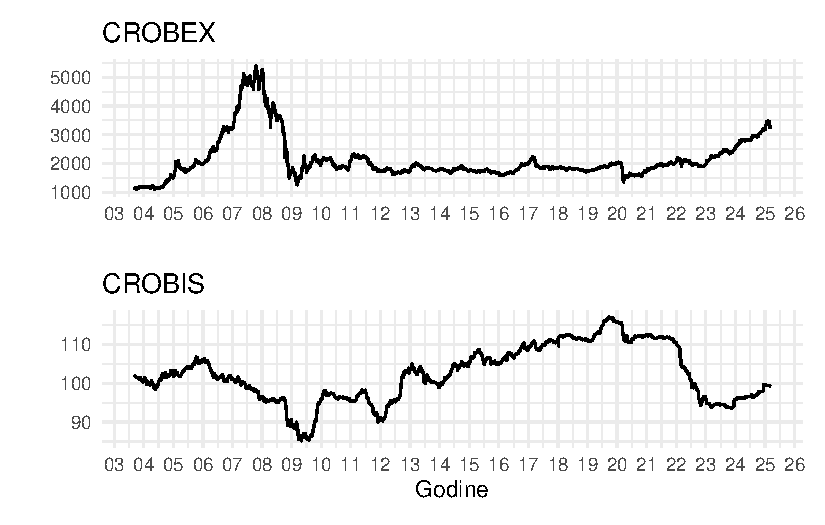
\includegraphics[keepaspectratio]{zse_eom_rebalansiranje_files/figure-pdf/fig-series-1.pdf}}

}

\caption{\label{fig-series}Dinamika CROBEX-a i CROBIS-a}

\end{figure}%

U radu se koriste dva vremenska niza: 1) CROBEX, koji odražava agregatnu
dinamiku dioničkog tržišta u RH 2) CROBIS, koji odražava dinamiku
obvezničkog tržišta u RH. Izvor podataka je Zagrebačka burza. Input
tablica sadrži tri kolone: simbol (CROBEX ili CROBIS), datum i
posljednja vrijednost indeksa na kraju dana. Raspon podataka je od
01.09.2003 do 07.03.2025. Vremenski nizovi CROBEX-a i CROBIS-a prikazani
su na slici Figure~\ref{fig-series}. Gornja slika pokazuje snažan rast
dionička tržišta u godinama koje su prethodile Velikoj Recesiji, te
snažan pad 2008 i 2009 godine. U sljedećih 25 godina CROBEX nije dosegao
najviše razine iz prethodnih razdoblja. Donja slika pokazuje dosta
drugačiju dinamiku obvezničkog tržišta. Obveznički indeks je padao u
razdoblju prije Velike Recesije, da bi potom, uslijed globalnog
smanjenja kamatnih stopa generirao pozitivne prinose sve do razdoblja
COVID-a. U 2022. godini CROBIS je snažno pao zbog rasta kamatnih stopa
uslijed inflacijskih pritisaka.

\begin{tabular}[t]{l|r|r|r|r|r|r}
\hline
symbol & N & Mean & Median & SD & Min & Max\\
\hline
crobex & 5335 & 3e-04 & 3e-04 & 0.0104 & -0.102 & 0.1593\\
\hline
crobis & 5335 & 0e+00 & 0e+00 & 0.0017 & -0.021 & 0.0212\\
\hline
\end{tabular}

Tablica (\textbf{tab-summary?}) prikazuje sažetak statistika za CROBEX i
CROBIS. U tablici se nalaze broj promatranja, prosječna vrijednost,
standardna devijacija, minimalna i maksimalna vrijednost dnevnih
prinosa. CROBEX pokazuje veću standardnu devijaciju i veći prinos, u
skladu s financijskom teorijom, prema kojoj dionice zbog rizične premije
imaju veće prinose i veći Minimalne i maksimalne vrijednosti indiciraju
deblje repove distribucije CROBEX prinosa.

U tablici (\textbf{tab-dep?}) su prikazane mjere povezanosti između
CROBEX-a i CROBIS-a. Sve tri korelacijske mjere (Pearson, Spearman,
Kendall) su iznimno niske, što upućuje na vrlo slabu međuovisnost
promatranih vremenskih nizova. Pearsonova korelacija odražava linearnu
vezu i vrlo je blizu nule, Spearmanova se odnosi na monotonu (rang)
povezanost i jednako tako ne pokazuje značajnije slaganje trendova, dok
Kendallova tau, koja mjeri omjer konkordantnih i diskordantnih parova,
također ukazuje na neznatnu ovisnost. Korelacije upućuju na to da se
CROBEX i CROBIS kreću neovisno jedan o drugom. Ovakva dinamika indicira
veću potencijalnu profitabilnost investicijske strategije koja kupuje
podcijenjenu imovinu, a prodaje precijenjenu imovinu.

\begin{tabular}[t]{r|r|r}
\hline
Pearson & Spearman & Kendall\\
\hline
0.0283 & 0.0186 & 0.0125\\
\hline
\end{tabular}

Za utvrđivanje utjecaja rebalansiranja na kretanje indeksa CROBEX
(dionički indeks) i CROBIS (obveznički indeks), koristimo deskriptivnu
analizu, regresijsku analizu i pristup investicijske strategije. U
nastavku specificiramo regresijsku jednadžbu i opisujemo algoritam
investicijske strategije.

Regresijska jednadžba za procjenu kalendarskog efekta ima oblik:

\[Ret_{e} = \alpha + \beta_1 Ret_{b} + \delta' X_t + \epsilon_t\]

gdje je \(Ret_{e}\) razlika prinosa CROBEX-a i CROBIS-a zadnjih 5
trgovinskih dana u mjesecu, a \(Ret_{b}\) razlika prinosa CROBEX-a i
CROBIS-a prvih 15 dana u mjesecu. Koeficijent \(\beta_1\) mjeri utjecaj
razlike prinosa prvih 15 dana u mjesecu na razliku prinosa zadnjih 5
dana u mjesecu. Ako je \(\beta_1\) statistički značajan i negativan, to
ukazuje na postojanje kalendarskog efekta. Matrica \(X_t\) sadrži
kontrolne varijable, koji mogu utjecati na dinamiku prinosa. U radu se
kao kontrolne varijable koriste mjesečni i godišnji jednostavni
momentumi. Na kraju, \(\varepsilon_{t}\) predstavlja greške modela i
obuhvaća sve ostale, neobjašnjene varijacije u prinosima.

Osim regresijske jednadžbe, kalendarski efekt rebalansiranja analizira
se i simuliranjem investicijske strategije. Strategija pretpostavlja
mjesečno rebalansiranje fondova u posljednjih pet trgovačkih dana u
mjesecu, prema sljedećem pravilu:

\begin{enumerate}
\def\labelenumi{\arabic{enumi})}
\tightlist
\item
  Prvo se izračunava razlika u kumulativnim dnevnim prinosima indeksa
  tijekom prethodnih 15 dana:
\end{enumerate}

\[RelR_{t} = \sum_{i=t-15}^{t-1} (R_i^{CROBEX} - R_i^{CROBIS})\]

\begin{enumerate}
\def\labelenumi{\arabic{enumi})}
\setcounter{enumi}{1}
\tightlist
\item
  Zatim se portfelj rebalansira prema pravilu:
\end{enumerate}

\[
Portfelj_{t} = 
\begin{cases}
\text{kupi CROBEX}, & \text{ako je } RelR_{t} > 0 \\[6pt]
\text{kupi CROBIS}, & \text{ako je } RelR_{t} \leq 0
\end{cases}
\]

Ako je razlika prinosa CROBEX-a i CROBIS-a pozitivna, kupuje se CROBEX,
a ako je negativna, kupuje se CROBIS. Portfelj se zadržava sljedećih pet
trgovačkih dana (do kraja mjeseca), nakon čega se ponovno provodi ista
procedura rebalansiranja. Ovakav pristup omogućuje iskorištavanje
kratkoročnih odstupanja cijena koja mogu nastati zbog aktivnosti
institucionalnih investitora pri mjesečnom rebalansiranju.

Portfolio se dakle sastoji samo od duge pozicije u jednoj imovini
(CROBEX ili CROBIS). U analizama investicijske strategije na temelju
sortiranja portfolia, često se koristi kombinacija duge i kratke
pozicije. To bi značilo zauzimanje kratke pozicije u precijenjenoj
imovini. Međutim, u radu se ne koristi duga pozicija, jer kratka prodaja
dionica nije moguća na Zagrebačkoj burzi.

Rezultati investicijske strategije prikazuju se s pomoću krivulje
kapitala i mjerama performansi portfolia. Od performansi se koriste
Sharpeov omjer, anualizirani prinos i maksimalni pad (drawdown).
Sharpeov omjer mjeri omjer prinosa i rizika, anualizirani prinos mjeri
prosječni godišnji prinos, a maksimalni pad mjeri najveći pad portfolia
u odnosu na prethodni maksimum.

\section{Rezultati}\label{rezultati}

U ovom se poglavlju analiziraju kalendarski efekti rebalansiranja. Ako
investicijski fondovi, koji ulažu u RH prilagođavaju udjele dionica i
obveznica u portfelju krajem mjeseca, efekt bi trebao imati utjecaj na
prinose krajem mjeseca. Prvo se provodi deskriptivna analiza, kako bi se
grafički procijenio efekt rebalansiranja na kraju mjeseca. U drugom
dijelu se provodi jednostavna regresijska analiza, kako bi se procijenio
utjecaj prinosa u prvom dijelu mjeseca na prinose u posljednjem tjednu
istog mjeseca. U trećem potpoglavlju se simulira investicijska
strategija, koja kupuje i drži podcijenjenu imovinu 5 dana prije kraja
mjeseca.

\subsection{Desktiptivna analiza}\label{desktiptivna-analiza}

\begin{figure}

\centering{

\pandocbounded{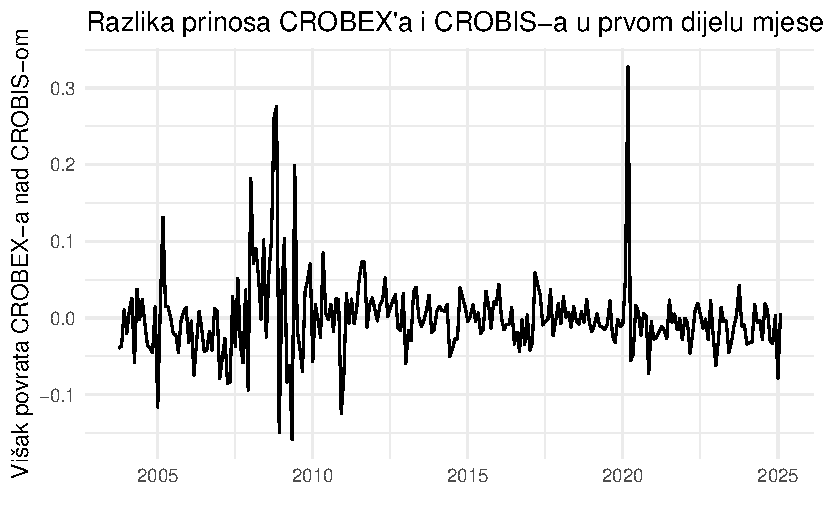
\includegraphics[keepaspectratio]{zse_eom_rebalansiranje_files/figure-pdf/fig-ratio-1.pdf}}

}

\caption{\label{fig-ratio}Razlika prinosa CROBEX'a i CROBIS-a u prvom
dijelu mjeseca}

\end{figure}%

Investicijski fondovi rebalansiraju portfolio ako se udio dionica ili
obveznica znatno odmakne od ciljanih udjela u portfoliju. Primjerice,
ako fond želi održavati fiksni udjel dionica i obveznica u omjeru 60/40,
te udio dionica tijekom mjeseca naraste na 62 \%, fond će krajem mjeseca
prodavati dionice i kupovati obveznice.

Na slici Figure~\ref{fig-ratio} je prikazana razlika prinosa CROBEX-a i
CROBIS-a u prvom dijelu mjeseca (oko 15 trgovinskih dana). Vrijednost
omjera iznad nule označava veći rast CROBEX-a u prvom dijelu mjeseca, i
obrnuto. U radu se analizira postoji li pritisak na pad vrijednosti
omjera za veće odmake od 0. Efekt se može jednostavno analizirati
izračunom prosječnog i medijalnog prinosa CROBEX-a kada je vrijednost
omjera veća od 0 ili manja od 0.

Slika Figure~\ref{fig-bar-mean} pokazuje razliku u prinosima CROBEX-a u
zadnjem tjednu u dva slučaja. Lijevi stupac na oba grafikona prikazuje
prinos CROBEX-a kada je prinos CROBEX-a u prvom dijelu tjedna bio manji
od prinosa CROBIS-a. Desna strana oba grafikona prikazuje prinose
CROBEX-a u svim zadnjim tjednima. Grafička analizira indicira postojanje
kalendarskog efekta jer su prinosi otprilike pola posto veći, ako se
uvjetuju razlikom između CROBEX-a i CROBIS-a u prvom dijelu mjeseca.
Efekt je izražen kako kod prosječnih, tako i kod medijalnih prinosa.

Slika Figure~\ref{fig-bar-crobis} pokazuje istu analizu za CROBIS. Na X
osi je dummy varijabla koja pokazuje uzimaju li se u obzir razlika
prinosa u prvom dijelu mjeseca. Graf ponovno pokazuje veće prinose
CROBIS-a, ako su uvjetovani disbalans CROBEX-a i CROBIS-a u prvom dijelu
mjeseca. Na lijevom grafu se vidi da su prosječni prinosi CROBIS-a
negativni ako se gledaju svi posljednji tjedni u mjesecu i pozitivni ako
se u obzir uzmu samo dani kod kojih je prinos CROBEX-a u odnosu na
CROBIS u prvom dijelu mjeseca bio pozitivan. Isti zaključak se može
donijeti i za medijalne prinose.

\begin{figure}

\centering{

\pandocbounded{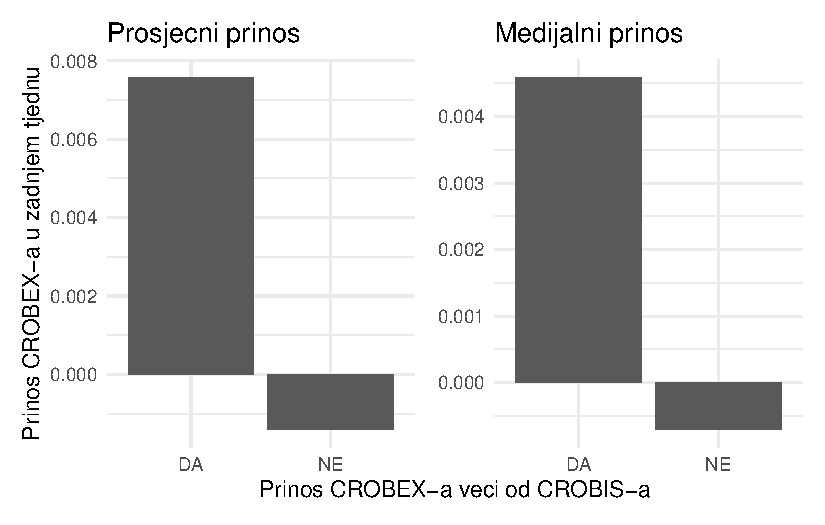
\includegraphics[keepaspectratio]{zse_eom_rebalansiranje_files/figure-pdf/fig-bar-mean-1.pdf}}

}

\caption{\label{fig-bar-mean}Prosječni i medijalni prinosi CROBEX-a u
zadnjem tjednu}

\end{figure}%

\begin{figure}

\centering{

\pandocbounded{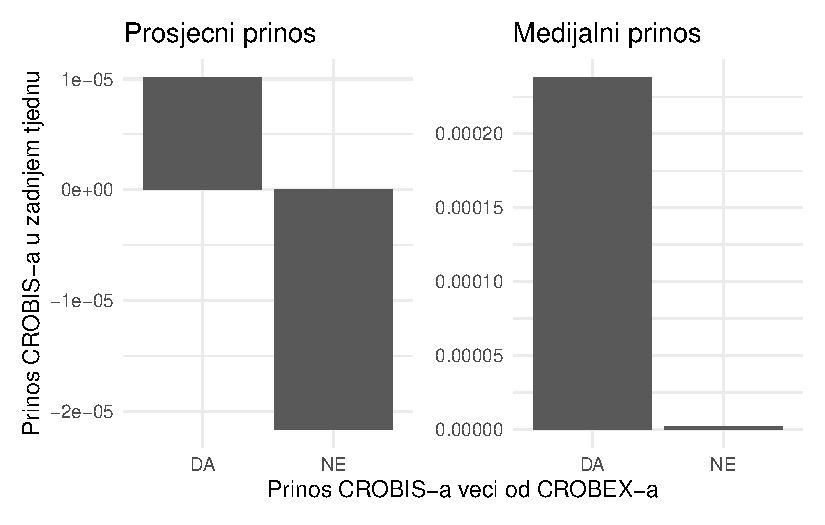
\includegraphics[keepaspectratio]{zse_eom_rebalansiranje_files/figure-pdf/fig-bar-crobis-1.pdf}}

}

\caption{\label{fig-bar-crobis}Prosječni i medijalni prinosi CROBIS-a u
zadnjem tjednu}

\end{figure}%

\subsection{Kalendarski efekt - pristup regresijske
analize}\label{kalendarski-efekt---pristup-regresijske-analize}

Započinjemo s vrlo jednostavnom regresijskom analizom. Zavisna varijabla
je višak prinosa CROBEX-a nad CROBIS-om u zadnjem tjednu tekućeg mjeseca
(od 16 trgovinskog dana do kraja mjeseca), a nezavisna varijabla je
višak prinosa CROBEX-a nad CROBIS-om u prvom dijelu mjeseca (od 1 do 15.
trgovinskog dana). Očekuje se negativna korelacija zavisne i nezavisne
varijable. Ako je CROBEX rastao više u prvom dijelu mjeseca, očekuje se,
u prosjeku, smanjenje viška prinosa u odnosu na CROBIS u drugom dijelu
mjeseca. U drugoj specifikaciji će se regresijska analiza proširiti za
dvije kontrolne varijable: mjesečni i godišnji momentum CROBEX-a i
CROBIS-a.

\begin{figure}

\centering{

\pandocbounded{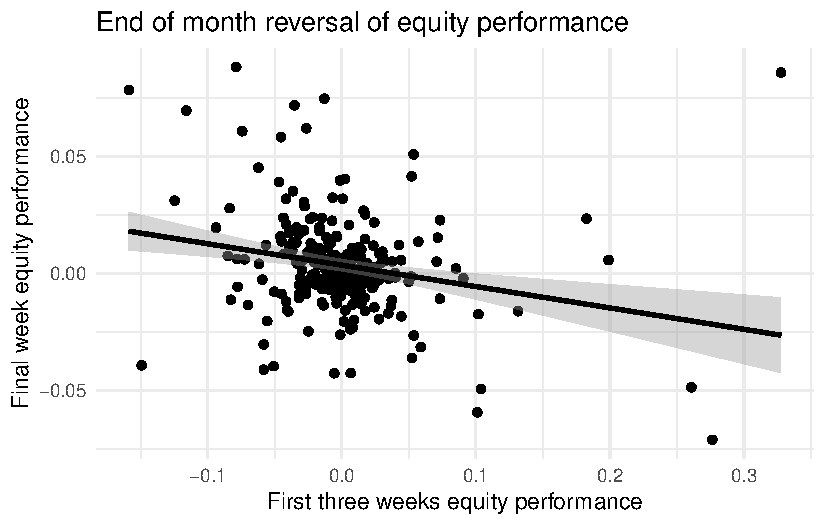
\includegraphics[keepaspectratio]{zse_eom_rebalansiranje_files/figure-pdf/fig-calendar-reg-1.pdf}}

}

\caption{\label{fig-calendar-reg}Dijagram raspršenosti razlike prinosa
CROBEX-a nad CROBIS-om i jednostavna linerna regresija razlike prinosa u
zadnjem tjednu na razliku prinosa u prvom dijelu mjeseca}

\end{figure}%

Slika Figure~\ref{fig-calendar-reg} prikazuje dijagram raspršenosti
razlike prinosa CROBEX-a i CROBIS-a u zadnjem dijelu mjeseca na y osi i
za prvi dio mjeseca na x osi. Slika pokazuje očekivano negativan nagib
regresijskog pravca. U posljednjem tjednu mjeseca događa povratak od
viših razlika prinosa prema nižim.

\begin{table}
\centering
\begin{talltblr}[         %% tabularray outer open
entry=none,label=none,
note{}={+ p \num{< 0.1}, * p \num{< 0.05}, ** p \num{< 0.01}, *** p \num{< 0.001}},
note{ }={Tablica prikazuje procjene regresijskih koeficijenata i standardne greške specifikacije dane u 1.},
]                     %% tabularray outer close
{                     %% tabularray inner open
colspec={Q[]Q[]Q[]Q[]Q[]},
column{2,3,4,5}={}{halign=c,},
column{1}={}{halign=l,},
hline{10}={1,2,3,4,5}{solid, black, 0.05em},
}                     %% tabularray inner close
\toprule
& LM 1 & LM 2 & LM HAC 1 & LM HAC 2 \\ \midrule %% TinyTableHeader
(Intercept) & \num{0.004}** & \num{0.003}* & \num{0.004}** & \num{0.003}* \\
& \num{0.001} (\num{0.005}) & \num{0.001} (\num{0.012}) & \num{0.001} (\num{0.007}) & \num{0.001} (\num{0.013}) \\
ratio\_1 & \num{-0.091}*** & \num{-0.089}*** & \num{-0.091} & \num{-0.089} \\
& \num{0.025} (\num{<0.001}) & \num{0.025} (\num{<0.001}) & \num{0.073} (\num{0.214}) & \num{0.075} (\num{0.233}) \\
mom\_month &  & \num{-0.000} &  & \num{-0.000} \\
&  & \num{0.000} (\num{0.717}) &  & \num{0.000} (\num{0.620}) \\
mom\_year &  & \num{0.000} &  & \num{0.000} \\
&  & \num{0.000} (\num{0.134}) &  & \num{0.000} (\num{0.338}) \\
Num.Obs. & \num{257} & \num{245} & \num{257} & \num{245} \\
R2 & \num{0.051} & \num{0.063} & \num{0.051} & \num{0.063} \\
R2 Adj. & \num{0.048} & \num{0.051} & \num{0.048} & \num{0.051} \\
AIC & \num{-1259.3} & \num{-1203.8} & \num{-1259.3} & \num{-1203.8} \\
BIC & \num{-1248.7} & \num{-1186.3} & \num{-1248.7} & \num{-1186.3} \\
Log.Lik. & \num{632.657} & \num{606.890} & \num{632.657} & \num{606.890} \\
F & \num{13.780} & \num{5.392} & \num{1.552} & \num{1.308} \\
RMSE & \num{0.02} & \num{0.02} & \num{0.02} & \num{0.02} \\
Std.Errors & IID & IID & HC3 & HC3 \\
\bottomrule
\end{talltblr}
\end{table}

Nakon grafičkog prikaza prikazujemo, u tablici
(\textbf{tab-calendar-reg?}) prikazujemo rezultate procjene parametara
regresijske jednadžbe. Prve dvije kolone prikazuju rezultate pod
pretpostavkom homoskedastičnih grešaka (LM 1 i LM 2), dok se u trećem i
četvrtom stupcu tablice prikazuju standardne pogreške prilagođene za
heteroskedastičnost. U tablici se prikazuju procjene regresijskih
koeficijenata, standardne greške procjene i zvjezdice koje označavaju
statističku značajnost koeficijenata. U koloni LM 1 se može vidjeti da
je koeficijent \(\beta_1\) statistički značajan i negativan, što upućuje
na postojanje kalendarskog efekta. U drugoj specifikaciji, koja
uključuje kontrolne varijable, koeficijent \(\beta_1\) zadržava
negativan predznak. Međutim, u kolonama LM HAC 1 i LM HAC 2, kod kojih
se koriste robusne standardne greške, koeficijent gubi statističku
značajnost.

Dijagram raspršenosti s regresijskim pravcem otkriva jednu neobičnu
opservaciju. Za bolji uvid o mogućoj značajnosti ove opservacije na
slici Figure~\ref{fig-calendar-residuals} prikazujemo rezidualne
vrijednosti regresijskog modela. Na slici se vidi da postoji jedna
opservacija koja se znatno odvaja od ostalih. Kako bi ispitali
osjetljivost modela na isključivanje ove opservacije, prikazujemo
rezultate regresijske analize bez ove opservacije. U tablici
(\textbf{tab-calendar-reg-outlier?}) prikazujemo rezultate regresijske
analize bez tog opažanja.

\begin{figure}

\centering{

\pandocbounded{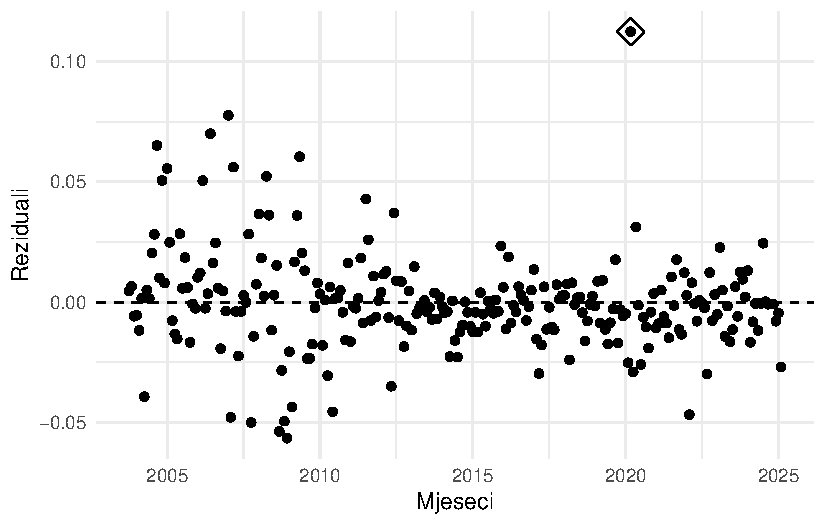
\includegraphics[keepaspectratio]{zse_eom_rebalansiranje_files/figure-pdf/fig-calendar-residuals-1.pdf}}

}

\caption{\label{fig-calendar-residuals}Reziduali regresijskog modela}

\end{figure}%

Rezultat regresijske analize bez jedne opservacije pokazuje statički
signifikantne koeficijente u svim kolonama. Koeficijent \(\beta_1\) je
negativan i statistički značajan uz razine značajnosti od 0.1 \%. Ovi
rezultati potvrđuju postojanje kalendarskog efekta u dinamici razlike
prinosa CROBEX-a i CROBIS-a.

\begin{table}
\centering
\begin{talltblr}[         %% tabularray outer open
entry=none,label=none,
note{}={+ p \num{< 0.1}, * p \num{< 0.05}, ** p \num{< 0.01}, *** p \num{< 0.001}},
note{ }={Tablica prikazuje procjene regresijskih koeficijenata i standardne greške specifikacije dane u 1.},
]                     %% tabularray outer close
{                     %% tabularray inner open
colspec={Q[]Q[]Q[]Q[]Q[]},
column{2,3,4,5}={}{halign=c,},
column{1}={}{halign=l,},
hline{10}={1,2,3,4,5}{solid, black, 0.05em},
}                     %% tabularray inner close
\toprule
& LM 1 & LM 2 & LM HAC 1 & LM HAC 2 \\ \midrule %% TinyTableHeader
(Intercept) & \num{0.003}** & \num{0.003}* & \num{0.003}* & \num{0.003}* \\
& \num{0.001} (\num{0.010}) & \num{0.001} (\num{0.018}) & \num{0.001} (\num{0.010}) & \num{0.001} (\num{0.020}) \\
ratio\_1 & \num{-0.153}*** & \num{-0.152}*** & \num{-0.153}*** & \num{-0.152}*** \\
& \num{0.025} (\num{<0.001}) & \num{0.025} (\num{<0.001}) & \num{0.043} (\num{<0.001}) & \num{0.043} (\num{<0.001}) \\
mom\_month &  & \num{0.000} &  & \num{0.000} \\
&  & \num{0.000} (\num{0.914}) &  & \num{0.000} (\num{0.863}) \\
mom\_year &  & \num{0.000} &  & \num{0.000} \\
&  & \num{0.000} (\num{0.299}) &  & \num{0.000} (\num{0.470}) \\
Num.Obs. & \num{256} & \num{244} & \num{256} & \num{244} \\
R2 & \num{0.129} & \num{0.142} & \num{0.129} & \num{0.142} \\
R2 Adj. & \num{0.126} & \num{0.132} & \num{0.126} & \num{0.132} \\
AIC & \num{-1290.9} & \num{-1235.5} & \num{-1290.9} & \num{-1235.5} \\
BIC & \num{-1280.3} & \num{-1218.0} & \num{-1280.3} & \num{-1218.0} \\
Log.Lik. & \num{648.466} & \num{622.751} & \num{648.466} & \num{622.751} \\
F & \num{37.708} &  & \num{12.826} &  \\
RMSE & \num{0.02} & \num{0.02} & \num{0.02} & \num{0.02} \\
Std.Errors & IID & IID & HC3 & HC3 \\
\bottomrule
\end{talltblr}
\end{table}

\subsection{Kalendarski efekt - pristup investicijske
strategije}\label{kalendarski-efekt---pristup-investicijske-strategije}

Ekonomski značaj kalendarskog efekta može se analizirati simulacijom
investicijske strategije, koja kupuje podcijenjenu imovinu 5 dana prije
kraja mjeseca. Ako je razlika prinosa CROBEX-a i CROBIS-a u prvom dijelu
mjeseca veća od 0, strategija kupuje CROBIS, a ako je razlika manja od
0, kupuje CROBEX.

Na slici Figure~\ref{fig-strategy} prikazan je grafikon prinosa
investicijske strategije. Na slici se vidi da je strategija donijela
veće prinose od oba indeksa.

\begin{figure}

\centering{

\pandocbounded{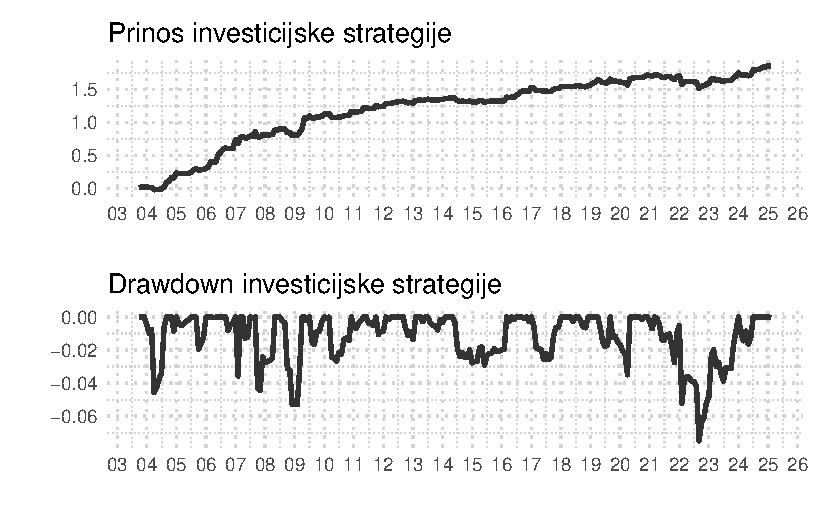
\includegraphics[keepaspectratio]{zse_eom_rebalansiranje_files/figure-pdf/fig-strategy-1.pdf}}

}

\caption{\label{fig-strategy}Prinos investicijske strategije}

\end{figure}%

\begin{tabular}[t]{l|r|r|r}
\hline
Mjera performansi & Kalendar & CROBEX & CROBIS\\
\hline
Anualizirani Sharpeov omjer & 0.8834492 & 0.3274513 & -0.0399463\\
\hline
Anualizirani prinos & 0.0502105 & 0.0539673 & -0.0011015\\
\hline
Drawdown & -0.0749996 & -0.7658828 & -0.2022041\\
\hline
\end{tabular}

Tablica (\textbf{tab-strategy?}) prikazuje performanse investicijske
strategije u usporedbi s performansama CROBEX-a i CROBIS-a. Strategija
je donijela veće prinose od oba indeksa. Sharpeov omjer strategije je
0.88, što je znatno veće od Sharpovog omjera CROBEX-a i CROBIS-a. Prinos
strategije je isti kao i prinos CROBEX-a, ali je rizik znatno manji.
Najveći pad CROBEX-a tijekom promatranog razdoblja je 76 \%, dok je
najveći gubitak strategije od ATH (eng. \emph{all time high}) 7.5 \%.

Budući da je strategija većinu vremena drži gotovinu, moguće je dodati
kamatnu stopu na gotovinu, kako bi se dobio ukupni nominalni prinos za
promatrano razdoblje. Ako se zada konzervativna kamatna stopa od 0.1 \%
mjesečno, Sharpeov omjer raste na 0.9.

Rezultati investicijske strategije nisu sasvim realni jer ne uključuju
transakcije troškove trgovanja. U analizi investicija, troškovi
trgovanja moraju biti uključeni u procjenu performansi portfolia.
Uključivanje fiksnih troškova trgovanja obuhvaća brokerske naknade,
\emph{bis/ask spreadove}, tržišni utjecaj, poreze i druge troškove.
Ignoriranje ovih troškova u nekim slučajevima može dovesti do
iskrivljenog prikaza stvarne performanse portfolia, što može ugroziti
točnost investicijskih odluka. Stoga u nastavku pokazujemo rezultate
strategije uz jednostavnu pretpostavku da investitor plaća fiksnu
naknadu trgovanja, koja iznosi c=0.1 \% za svaku transakciju. Budući da
krajem mjeseca kupujemo i prodajemo CROBEX ili CROBIS, ukupni trošak
trgovanja je 0.2 \% mjesečno. Tablica (\textbf{tab-strategy-costs?})
prikazuje performanse investicijske strategije uz troškove trgovanja.
Prinosi su znatno manji, ali je Sharpeov omjer još uvijek veći od
CROBEX-a i CROBIS-a.

\begin{tabular}[t]{l|r|r|r}
\hline
Mjera performansi & Kalendar & CROBEX & CROBIS\\
\hline
Anualizirani Sharpeov omjer & 0.4465262 & 0.3274513 & -0.0399463\\
\hline
Anualizirani prinos & 0.0253781 & 0.0539673 & -0.0011015\\
\hline
Drawdown & -0.1477502 & -0.7658828 & -0.2022041\\
\hline
\end{tabular}

\section{Analiza robusnosti}\label{analiza-robusnosti}

\subsection{Kalendarski efekt početkom
mjeseca}\label{kalendarski-efekt-poux10detkom-mjeseca}

Kalendarski efekt je analiziran uvjetovanjem razlike prinosa CROBEX-a i
CROBIS-a u zadnjem tjednu na višak prinosa u prvom dijelu mjeseca. U
ovom dijelu analize se provjerava postoji li isti efekt, ako se kao prvi
period gleda prinos u zadnja tri tjedna u mjesecu, a kao drugi period
prvi tjedan u sljedećem mjesecu. Ako investicijski fondovi rebalansiraju
portfelje na početku mjeseca, očekuje se da će razlika prinosa CROBEX-a
i CROBIS-a u prvom dijelu mjeseca imati utjecaj na razliku prinosa u
zadnjem dijelu mjeseca. Istovremeno se ispituje postoji predviđa li
prinos u tri tjedna generalno prinos u sljedećem tjednu. Ako je to
slučaj, to bi moglo ukazivati da signifikantni kalendarski efekt nije
posljedica rebalansiranja portfelja, već nekog drugog faktora. Kao i u
prethodnom poglavlju, provodi se regresijska analiza i investicijska
strategija.

\begin{table}
\centering
\begin{talltblr}[         %% tabularray outer open
entry=none,label=none,
note{}={+ p \num{< 0.1}, * p \num{< 0.05}, ** p \num{< 0.01}, *** p \num{< 0.001}},
note{ }={Tablica prikazuje procjene regresijskih koeficijenata i standardne greške specifikacije dane u 1.},
]                     %% tabularray outer close
{                     %% tabularray inner open
colspec={Q[]Q[]Q[]},
column{2,3}={}{halign=c,},
column{1}={}{halign=l,},
hline{6}={1,2,3}{solid, black, 0.05em},
}                     %% tabularray inner close
\toprule
& LM 1 & LM HAC 1 \\ \midrule %% TinyTableHeader
(Intercept) & \num{0.000} & \num{0.000} \\
& \num{0.001} (\num{0.834}) & \num{0.001} (\num{0.839}) \\
ratio\_1 & \num{0.070}* & \num{0.070} \\
& \num{0.031} (\num{0.023}) & \num{0.067} (\num{0.300}) \\
Num.Obs. & \num{256} & \num{256} \\
R2 & \num{0.020} & \num{0.020} \\
R2 Adj. & \num{0.016} & \num{0.016} \\
AIC & \num{-1210.2} & \num{-1210.2} \\
BIC & \num{-1199.5} & \num{-1199.5} \\
Log.Lik. & \num{608.081} & \num{608.081} \\
F & \num{5.253} & \num{1.081} \\
RMSE & \num{0.02} & \num{0.02} \\
Std.Errors & IID & HC3 \\
\bottomrule
\end{talltblr}
\end{table}

Tablica (\textbf{tab-calendar-reg-start?}) prikazuje rezultate
regresijske analize kalendarskog efekta, gdje se kao prvi period uzima
prinos u zadnja tri tjedna u mjesecu, a kao drugi period prvi tjedan u
sljedećem mjesecu. Prvo se može primijetiti da je vrijednost
koeficijenta upola manja u odnosu na bazičnu specifikaciju. Koeficijent
ima i obrnuti smjer, odnosno koeficijent \(\beta_1\) je pozitivan. Pod
pretpostavkom homoskedastičnosti, koeficijent je statistički
signifikantan, ali uz mnogo manju razinu značajnosti u odnosu na bazični
model. Ako se koriste robusne standardne pogreške, koeficijent postaje
statistički nesignifikantan.

Slika Figure~\ref{fig-strategy-start} prikazuje performanse
investicijske strategije, koja kupuje podcijenjenu imovinu na početku
mjeseca. Na slici se jasno vidi da strategije ostvaruje vrlo loše
rezultate. Strategije je tijekom cijelog mjeseca izgubila više od 10 \%
vrijednosti i u kontinuiranom je gubitku od 2007. godine.

\begin{figure}

\centering{

\pandocbounded{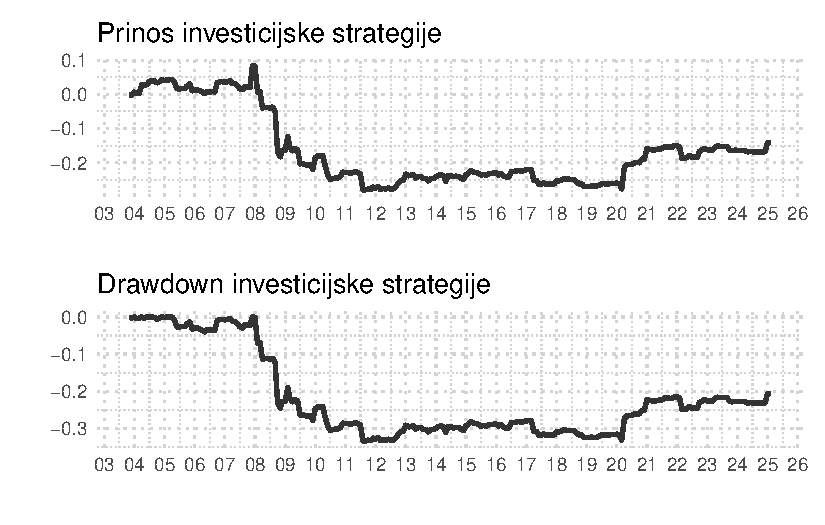
\includegraphics[keepaspectratio]{zse_eom_rebalansiranje_files/figure-pdf/fig-strategy-start-1.pdf}}

}

\caption{\label{fig-strategy-start}Prinos investicijske strategije}

\end{figure}%

\subsection{Osjetljivost rezultata na broj dana krajem
mjeseca}\label{osjetljivost-rezultata-na-broj-dana-krajem-mjeseca}

U bazičnom modelu, kao prvi datum za računanje prinosa u zadnjem tjednu
mjeseca uzet je 16. dan u mjesecu. U ovom dijelu analize se ispituje
osjetljivost rezultata na promjenu ovog dana. U analizi se uzimaju
različiti datumi, od 11. do 20. dana u mjesecu.

\pandocbounded{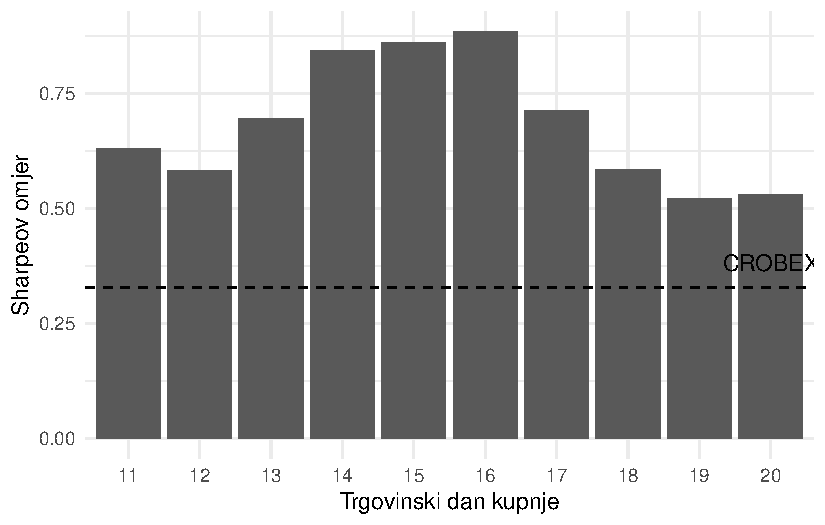
\includegraphics[keepaspectratio]{zse_eom_rebalansiranje_files/figure-pdf/unnamed-chunk-26-1.pdf}}

\section{Zaključak}\label{zakljuux10dak}

Rezultati istraživanja potvrđuju postojanje kalendarskog efekta
rebalansiranja na Zagrebačkoj burzi. Analiza pokazuje da institucionalni
investitori, posebno mirovinski fondovi, prilagođavaju udjele dionica i
obveznica u svojim portfeljima krajem mjeseca, što utječe na agregatna
tržišna kretanja. Regresijski modeli pokazuju negativan odnos razlike
prinosa dionica i obveznica u prvom dijelu mjeseca i razlike prinosa u
posljednjem tjednu, što upućuje na sistematski povratak cijena prema
ravnoteži. Nadalje, simulacija investicijske strategije temeljenje na
ovom efektu pokazuje superiorne performanse u usporedbi s jednostavnom
strategijom „kupi i drži``.

Analiza robusnosti dodatno potvrđuje nalaze, pri čemu se pokazuje da
sličan efekt ne postoji na početku mjeseca, što isključuje mogućnost da
je uočena pojava rezultat općih tržišnih trendova. Također, analiza
osjetljivosti na promjenu broja dana pokazuje da je investicijska
strategija robuisna na izbor ovog parametra.

Ovi rezultati imaju važne implikacije za investicijske fondove, koji bi
trebali razmotriti optimizaciju svojih rebalansiranja kako bi smanjili
troškove i tržišne utjecaje. Također, sofisticirani investitori mogu
koristiti ove nalaze za prilagodbu vlastitih strategija trgovanja.
Konačno, nalazi rada mogu poslužiti regulatorima i kreatorima politika
pri oblikovanju pravila upravljanja portfeljima u cilju poboljšanja
efikasnosti tržišta kapitala u Hrvatskoj.

Istraživanje ima nekoliko ograničenja. Procjena graničkog efekta
rebalansiranja je aproksimacija ponašanja investicijskih fondova. Iako
je u regresijsokj analizi efekt signifikantan i nakon dodavanja
kontrolnih varijabli, moguće je da postoji drugi uzroci uspješnosti
investicijske strategije ili signifikanstnosti parametara. Točan efekt
moguće je procijeniti samo uz podatke o rebalansiranju za sve
investicijske fondove. Riječ o alternativnim podacima koji su teško
dostupni, ali moguće je proširiti analizu u budućnosti s novim podacima.
Kalendarski efekt također može biti rezultat djelovanja drugih varijabli
iz takozvanih \emph{zoo} faktora, koje nisu uključene u analizu. Osim
toga, korišteni modeli pretpostavljaju linearnost odnosa između
promatranih varijabli, dok stvarni tržišni odnosi mogu biti nelinearni
ili podložni promjenama u različitim tržišnim režimima.

\phantomsection\label{refs}
\begin{CSLReferences}{1}{0}
\bibitem[\citeproctext]{ref-da2018destabilizing}
Da, Zhi, Borja Larrain, Clemens Sialm, and José Tessada. 2018.
{``Destabilizing Financial Advice: Evidence from Pension Fund
Reallocations.''} \emph{Review of Financial Studies} 31 (1): 1--43.
\url{https://doi.org/10.1093/rfs/hhy011}.

\bibitem[\citeproctext]{ref-Doe2025}
Doe, John. 2025. {``The Impact of Technology on Education.''}
\url{https://ssrn.com/abstract=5122748}.

\bibitem[\citeproctext]{ref-DundjekKokotec2021}
Đunđek Kokotec, Ivana, Silvije Orsag, and Marina Klačmer Čalopa. 2021.
{``The Impact of Institutional Investors' Ownership on Performance and
Financial Position: Evidence from Firms in the Republic of Croatia.''}
\emph{The South East European Journal of Economics and Business} 16 (1):
53--69. \url{https://doi.org/10.2478/jeb-2021-0005}.

\bibitem[\citeproctext]{ref-Etula2020}
Etula, Erik, Kim Rinne, Matti Suominen, and Lauri Vaittinen. 2020.
{``Dash for Cash: Monthly Market Impact of Institutional Liquidity
Needs.''} \emph{Review of Financial Studies} 33 (1): 75--111.
\url{https://doi.org/10.1093/rfs/hhz084}.

\bibitem[\citeproctext]{ref-harris1986}
Harris, Lawrence, and Eitan Gurel. 1986. {``Price and Volume Effects
Associated with Changes in the s\&p 500 List: New Evidence for the
Existence of Price Pressures.''} \emph{The Journal of Finance} 41 (4):
815--29. \url{https://doi.org/10.2307/2328230}.

\bibitem[\citeproctext]{ref-hanfa2025}
Hrvatska agencija za razvoj financijskih usluga (HANFA). 2025.
{``Mjesečni Pregled Sektora Financijskih Usluga - Siječanj 2025.''}
\url{https://www.hanfa.hr/media/phck4f1i/mjese\%C4\%8Dni-pregled-sfu-sije\%C4\%8Danj-2025.pdf}.

\bibitem[\citeproctext]{ref-ParkerSchoarSun2022}
Parker, Jonathan A., Antoinette Schoar, and Yang Sun. 2022. {``Retail
Financial Innovation and Stock Market Dynamics: The Case of Target Date
Funds.''} \emph{Journal of Finance, Forthcoming}.

\bibitem[\citeproctext]{ref-PengWang2024}
Peng, Cameron, and Chen Wang. 2024. {``Factor Rebalancing.''}

\bibitem[\citeproctext]{ref-shleifer1986}
Shleifer, Andrei. 1986. {``Do Demand Curves for Stocks Slope Down?''}
\emph{The Journal of Finance} 41 (3): 579--90.
\url{https://doi.org/10.2307/2328486}.

\end{CSLReferences}




\end{document}
